\subsection{Two-photon microscopy}
Two-photon microscopy is a fluorescence imaging technique, where two photons are brought to an excitation state at the same time and then absorbed to emit a photon of fluorescence. As the wavelength of the two excited photons is required to be longer than the emitted light, near-infrared excitation light is often used. Because of the multi photon absorption, the background signal is strongly suppressed, and because using infrared light minimizes scattering in tissue, two-photon microscopy gets an increased penetration depth over confocal microscopy, which uses a spatial pinhole technique to block out-of-focus light \cite{confocal}. Due to this increased penetration depth, two-photon microscopy can be used to obtain images of living tissue up to one millimetre in thickness \cite{wikimicroscopy}. For this project, this means two-photon microscopy can be used to measure transcytosis through the blood-brain barrier. This is done in \cite{imaging} where the change in blood-brain barrier permeability of small molecules is measured after injection of fluorophore, a compound which emits photons upon excitation. In more detail this was done by using two-photon microscopy in vivo in mice, where the anesthetized mice's brains were imaged through a craniotomy over the somatosensory cortex. The light emitting fluorophore signal can then be measured in both the blood vessels and brain parenchyma. The used two-photon microscopy allows for imaging at different depths in the tissue and can be compiled to a three dimensional reconstruction of the brain microvasculature. \autoref{puncta} shows a cross section of such reconstructions and thus how the transcytosis in the blood-brain barrier has been affected. With time, the fluorophore coalesce into numerous puncta of vescicles. In \autoref{puncta} we see these puncta of vesicles which accumulate around the blood-brain barrier interface. The three dimensional reconstruction can be sliced in different ways to give different perspectives of the results. Imagining the reconstruction as a block \autoref{puncta} is likely images where the block has been sliced from top to bottom. One could also slice the block from left to right giving a view of the 'insides' of the arteries where we would then see the puncta coalesce in a circle around the blood-brain barrier interface. 
%\begin{figure}[H]
%	\centering
%	\begin{subfigure}[b]{\linewidth}
%		\centering
%		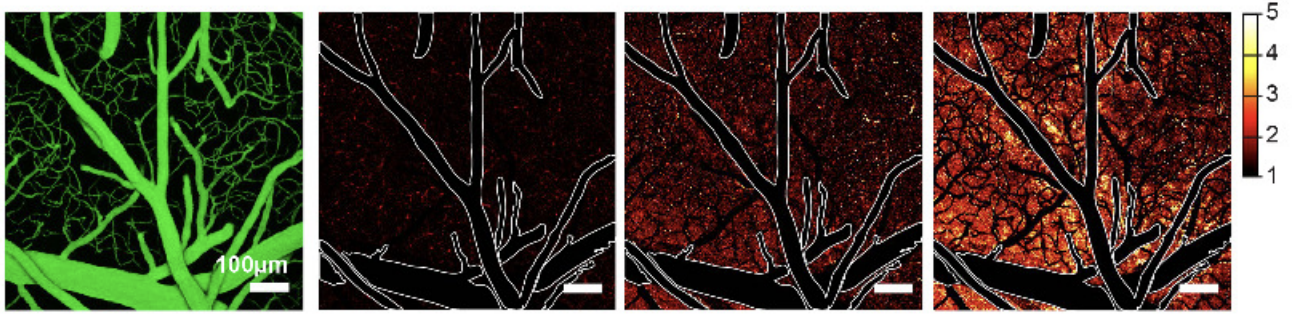
\includegraphics[width=0.9\linewidth]{Materials/Theory/paperres}
%		\caption{Cross section time lapse images with injection of NaFluo. We see an accumulation of NaFluo in the brain parenchyma over a period of 30 minutes. Image taken from \cite{imaging}.}
%		\label{paperres}
%	\end{subfigure}
%	\\
%	\begin{subfigure}[b]{\linewidth}
%		\centering
%		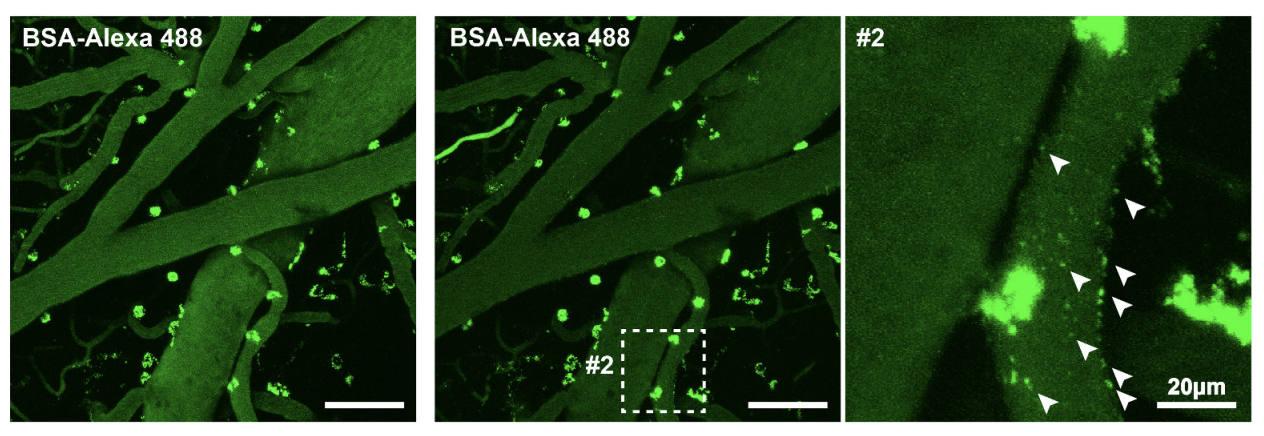
\includegraphics[width=0.7\linewidth]{Materials/Theory/puncta}
%		\caption{Coalescence of BSA-Alexa 488 after 60 and 120 minutes. White arrows indicate puncta we are interested in finding. Image taken from \cite{imaging}.}
%		\label{puncta}
%	\end{subfigure}
%\end{figure}
\begin{figure}
	\centering
	\begin{subfigure}[b]{0.2\linewidth}
		\centering
		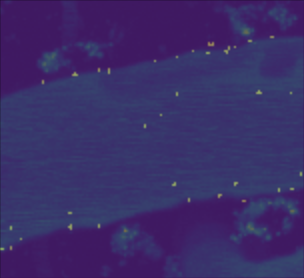
\includegraphics[width=\linewidth]{Materials/Theory/series1}
	\end{subfigure}
	\qquad
	\begin{subfigure}[b]{0.2\linewidth}
		\centering
		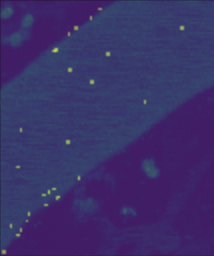
\includegraphics[width=0.77\linewidth]{Materials/Theory/series2}
	\end{subfigure}
	\qquad
	\begin{subfigure}[b]{0.2\linewidth}
		\centering
		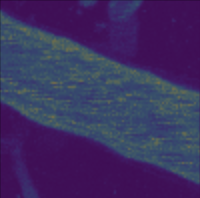
\includegraphics[width=0.94\linewidth]{Materials/Theory/series3}
	\end{subfigure}
	\caption{Cross section images of reconstruction taken from the training data and overlaid with the true masks indicating puncta we are interested in finding.}
	\label{puncta}
\end{figure}